\paragraph{i}
\begin{equation}
    \begin{split}
        v &= \frac{d}{t} \frac{A}{A} = \frac{V}{t}\frac{1}{A} \\
          &= \frac{ \SI{5e-6}{m^3.s^{-1}} }{ {(\SI{2e-3}{m})}^2 \pi } = \SI{0.40}{m.s^{-1}}
    \end{split}
\end{equation}

\paragraph{ii}
\begin{equation}
    f_{d} = \pm \frac{ 2vf \cos \theta }{ c }
\end{equation}
\begin{equation*}
    f_{da} = \frac{ 2\cdot 0.4 \cdot \num{5e6} \cdot 3/5 }{ 1540 } = +\SI{1558}{Hz}
\end{equation*}
\begin{equation*}
    f_{db} = 2 \cdot 0.40 \cdot \num{5e6} \cos(\pi/2) = 0
\end{equation*}
Analogously to $f_{da}$, $f_{dc} = -\SI{1558}{Hz}$

\paragraph{iii}
From the question we infer that at $t=0$, $\phi/2 = \tan^{-1} (3/4)$
\begin{equation}\begin{split}
    \frac{d\phi}{dt} = 26 \implies \phi = 26t + C\\
    \therefore \phi = 0.026t + 1.2870 \quad \text{ for $t$ in \si{ms}}
\end{split}
\end{equation}
Given that $\theta = \pi/2 - \phi/2 $, the equation for $f_d$ is plotted in Figure \ref{fig:doppler-variation}.

\begin{figure}[h]
    \centering
    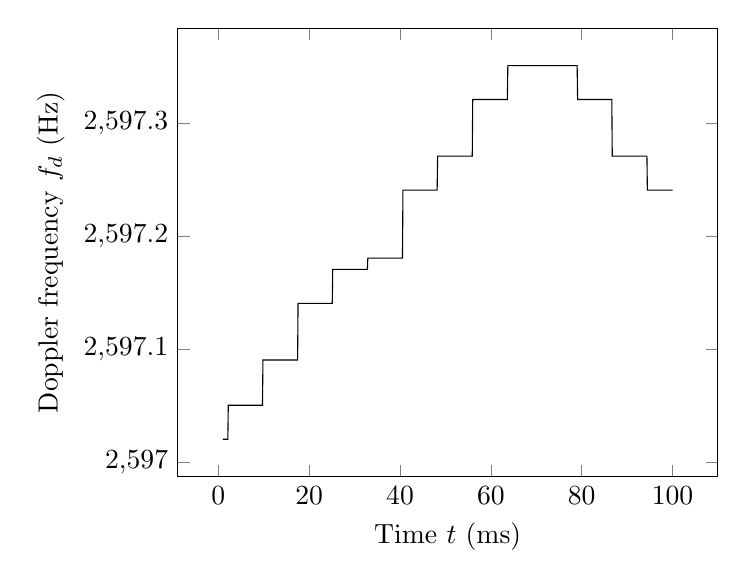
\begin{tikzpicture}
        \begin{axis}[xlabel=Time $t$ (\si{ms}), ylabel=Doppler frequency $f_d$ (\si{Hz})]
            \addplot[domain=1:100, samples=1000] {2*0.4*5000000*cos(pi/2 - (0.026*x+1.2870)/2 )/1540};
        \end{axis}
    \end{tikzpicture}
    \caption{Doppler frequency over a period of \SI{100}{ms}, starting from A.}
    \label{fig:doppler-variation}
\end{figure}

\paragraph{iv}
\begin{equation}
    Q = v_c^{'} A \implies v_c^{'} = \frac{\SI{5e-6}{m^3.s^{-1}}}{ {(\SI{1e-3}{m})}^2\pi } = \SI{1.5915}{m.s^{-1}}
\end{equation}
\begin{equation}
    f_{dc}^{'} = \pm \frac{ 2v^{'}_c f \cos \theta }{ c } = - \frac{1.5915 \cdot \num{5e6} \cdot 3/5}{1540} = - \SI{6200}{Hz}
\end{equation}